\documentclass[11pt]{article}
\usepackage[a4paper,margin=2cm]{geometry}
\usepackage{graphicx,booktabs,amsmath,float,caption}
\usepackage[hidelinks]{hyperref}
\setlength{\parskip}{4pt}\setlength{\parindent}{0pt}

\title{\textbf{PRML Lab 5 --- QDA, LDA, Gaussian MLE and Naive Bayes for Text}}
\author{Aryan Tiwari (B20AI056)\\CSL2050 Pattern Recognition \& Machine Learning, Winter 2022}
\date{}

\begin{document}
\maketitle

\section*{Question 1 --- QDA and LDA on Iris}

\textbf{A. Pre-processing and split.} 150 flowers, 4 features (cm), 3 balanced species, no missing values. The 3 duplicate rows are
genuine repeated measurements (values are rounded to 0.1 cm), so they are kept. QDA/LDA are not affected by rescaling the features, so no normalisation is needed.
70:30 split, \textbf{stratified}, so the test set has exactly 15 flowers of each species (105 train / 45 test).

\begin{figure}[H]\centering
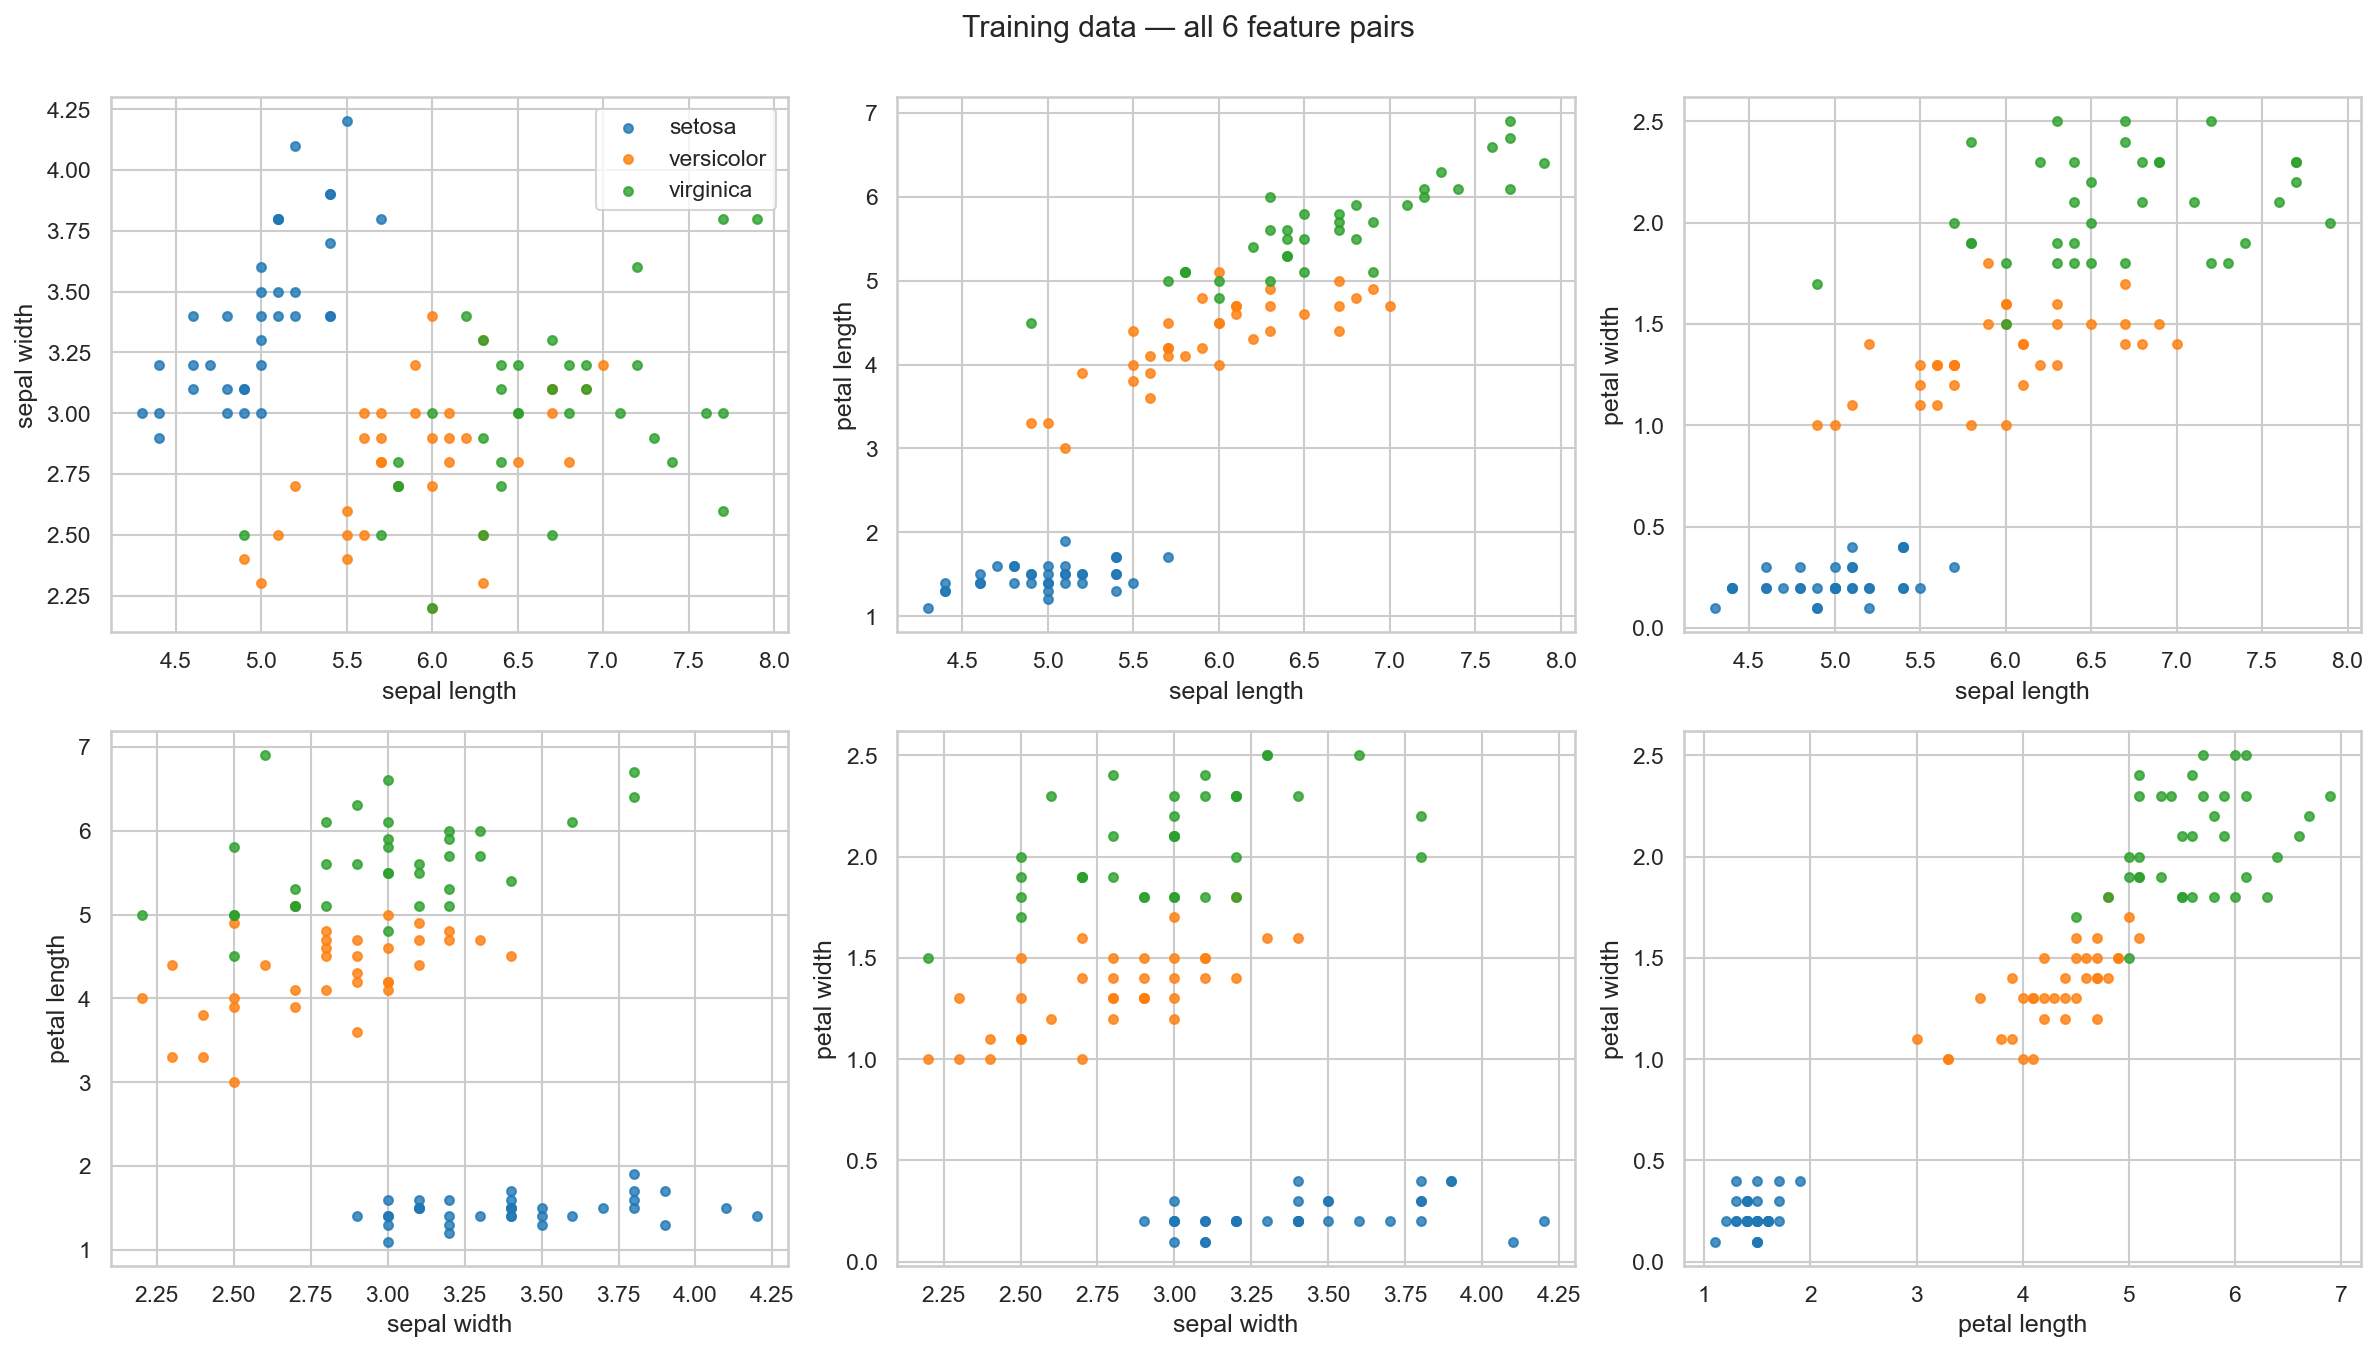
\includegraphics[width=0.92\linewidth]{figures/q1_pairs.png}
\caption{Training data for all six feature pairs. Setosa is always isolated; the petal features separate versicolor from virginica best.}
\end{figure}

\textbf{B. Feature pairs.} (1) \emph{petal length $\times$ petal width}: the tightest, most separated clusters;
(2) \emph{sepal length $\times$ petal length}: petal length does most of the work, and sepal length adds a second direction;
(3) \emph{sepal width $\times$ petal width}: petal width separates the species, and sepal width gives setosa a differently shaped
covariance, which is a good test of QDA's per-class covariances.

\textbf{C. QDA parameters} (mean $\mu$ and covariance $\Sigma$ per class):
\begin{table}[H]\centering\small
\begin{tabular}{llll}\toprule
Pair & Class & $\mu$ & $\Sigma$\\\midrule
petal L $\times$ petal W & setosa & (1.471, 0.229) & [[0.0239, 0.0035], [0.0035, 0.0068]]\\
 & versicolor & (4.311, 1.343) & [[0.2516, 0.0768], [0.0768, 0.0419]]\\
 & virginica & (5.631, 2.071) & [[0.3169, 0.0492], [0.0492, 0.0680]]\\\midrule
sepal L $\times$ petal L & setosa & (4.983, 1.471) & [[0.1173, 0.0233], [0.0233, 0.0239]]\\
 & versicolor & (5.960, 4.311) & [[0.2872, 0.2149], [0.2149, 0.2516]]\\
 & virginica & (6.643, 5.631) & [[0.4590, 0.3377], [0.3377, 0.3169]]\\\midrule
sepal W $\times$ petal W & setosa & (3.409, 0.229) & [[0.1179, 0.0106], [0.0106, 0.0068]]\\
 & versicolor & (2.806, 1.343) & [[0.0900, 0.0430], [0.0430, 0.0419]]\\
 & virginica & (2.989, 2.071) & [[0.1299, 0.0508], [0.0508, 0.0680]]\\\bottomrule
\end{tabular}
\end{table}

\textbf{D--E. Decision boundaries and test error.}
\begin{figure}[H]\centering
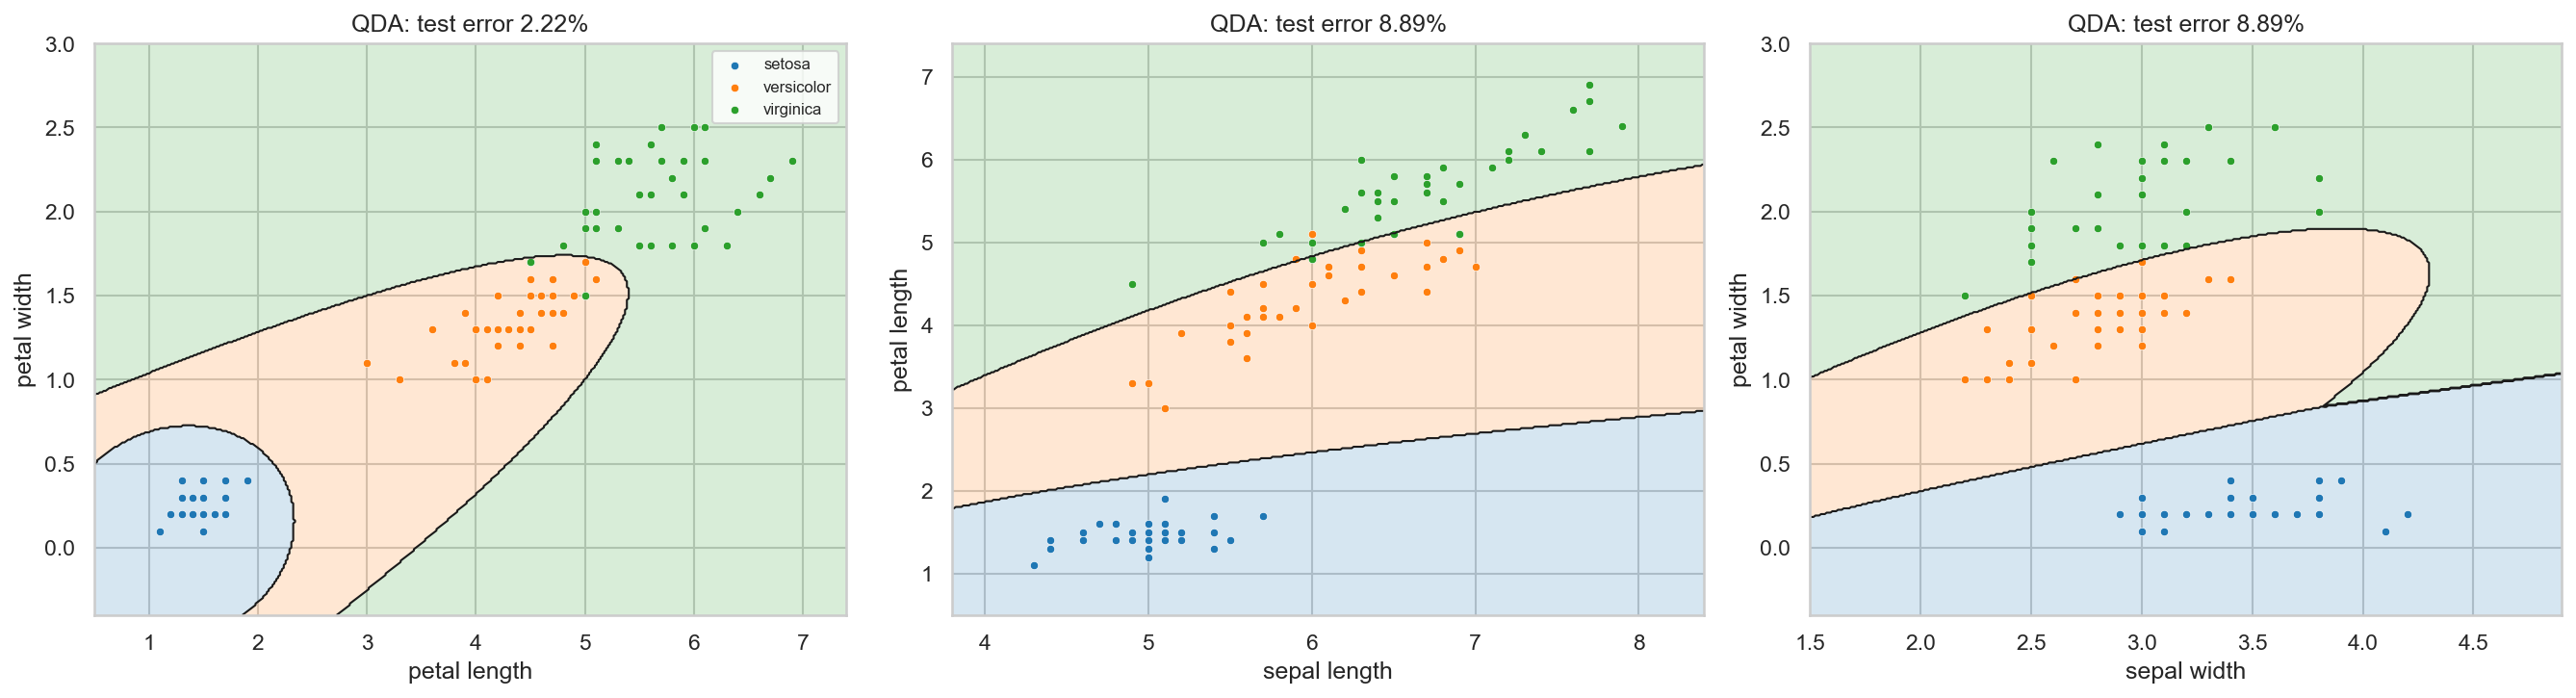
\includegraphics[width=\linewidth]{figures/q1_qda_boundaries.png}
\caption{QDA decision regions (curved boundaries) over the training data.}
\end{figure}

\begin{table}[H]\centering
\begin{tabular}{lccc}\toprule
Pair & Test error & Train error & Test log-loss\\\midrule
petal length $\times$ petal width & \textbf{2.22\%} (1/45) & 2.86\% & \textbf{0.076}\\
sepal length $\times$ petal length & 8.89\% (4/45) & 5.71\% & 0.156\\
sepal width $\times$ petal width & 8.89\% (4/45) & 1.90\% & 0.260\\\bottomrule
\end{tabular}
\end{table}
\textbf{Petal length $\times$ petal width is best.} Both features measure the petal, which is where the three species differ most. In this plane the
versicolor and virginica clouds barely overlap, so only one virginica is misclassified. The other two pairs each include a sepal feature,
and in sepal measurements versicolor and virginica overlap heavily. The third pair also shows overfitting: its training error is the lowest (1.9\%)
but its test log-loss is the worst, because QDA fits a separate curved boundary per class from only 35 samples each.

\textbf{F--H. LDA on the best pair.}
\begin{figure}[H]\centering
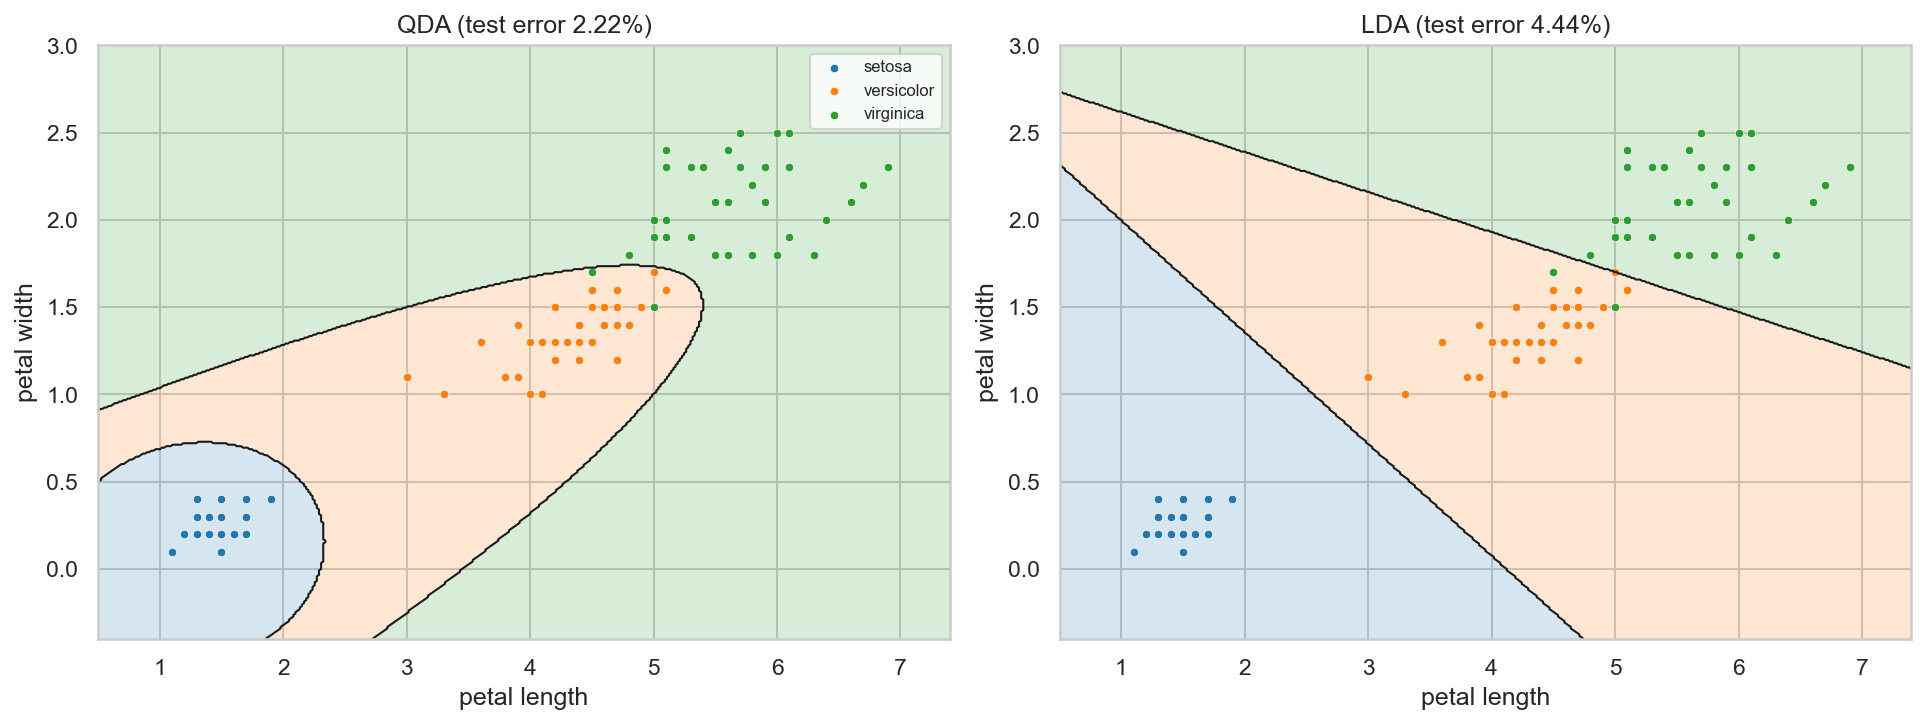
\includegraphics[width=0.85\linewidth]{figures/q1_lda_vs_qda.png}
\caption{QDA (curved) vs.\ LDA (straight) boundaries on petal length $\times$ petal width.}
\end{figure}

LDA gets a test error of \textbf{4.44\%} (2/45) compared with QDA's 2.22\%, with the same training error (2.86\%) and twice the
test log-loss (0.147 vs.\ 0.076). \textbf{QDA performs better here.} LDA assumes all classes share one covariance
($\Sigma = $ [[0.192, 0.042], [0.042, 0.038]]). That is clearly false for iris: setosa's petal covariance is roughly 10$\times$ smaller
than virginica's. Because of the shared covariance LDA's boundaries are straight lines, and the line between versicolor and virginica lies slightly off the
best cut. QDA estimates 15 covariance parameters instead of LDA's 9 (with means, 6 are common to both), and with 35 samples per class that
is still well supported. With much less data, LDA's lower variance could win.

\textbf{I. Fitted Gaussians.}
\begin{figure}[H]\centering
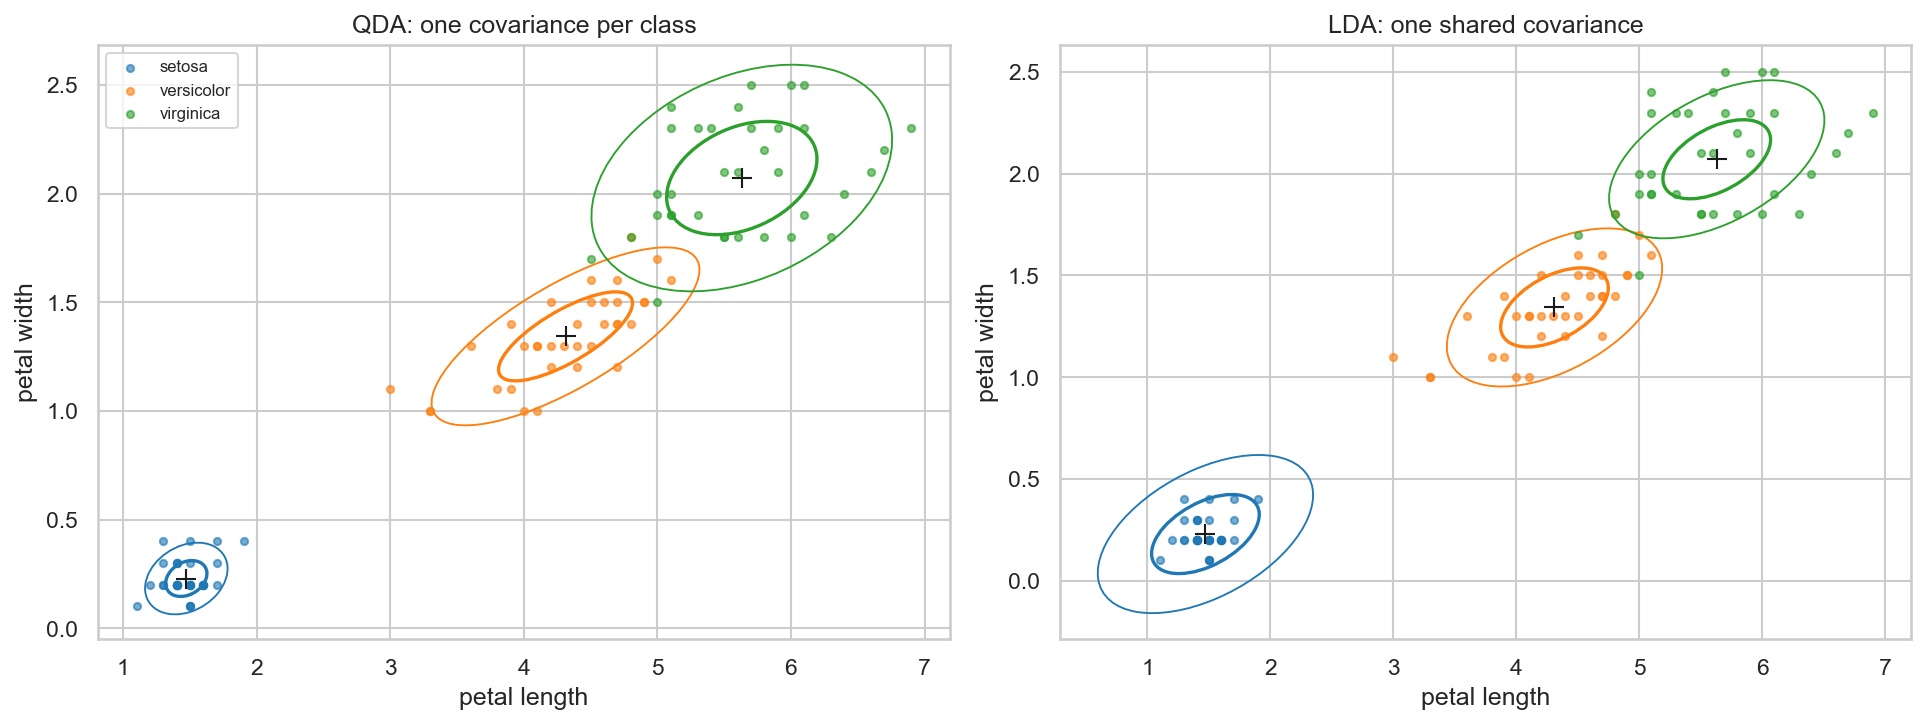
\includegraphics[width=0.9\linewidth]{figures/q1_gaussians.png}
\caption{1$\sigma$ and 2$\sigma$ ellipses. QDA (left) gives each species its own size and orientation; LDA (right) forces one shape on all three.}
\end{figure}

\section*{Question 2 --- Gaussian MLE and a Bayes classifier (petal length \& width)}

\textbf{a. Sample estimates.} Computed with the unbiased estimator $S = \frac{1}{n-1}\sum (x-\bar x)(x-\bar x)^\top$. They are identical to the
QDA parameters in Q1 (QDA uses the same estimator).

\textbf{b. \texttt{compute\_likelihood}.} The density
$\mathcal N(x;\mu,\Sigma) = (2\pi)^{-1}|\Sigma|^{-1/2}\exp(-\tfrac12 (x-\mu)^\top\Sigma^{-1}(x-\mu))$ is implemented from scratch,
with the $2\times2$ determinant and inverse written out by hand, plus a log version so that products of small densities don't underflow. It matches
\texttt{scipy.stats.multivariate\_normal} to within $4\times10^{-15}$.

\textbf{c. MLE and Bayes classifier.} Maximising the log-likelihood gives the sample mean and the \emph{biased} covariance
$\hat\Sigma = \frac1n\sum (x-\hat\mu)(x-\hat\mu)^\top$, which equals the sample covariance multiplied by $(n-1)/n = 0.971$ for $n=35$:

\begin{table}[H]\centering\small
\begin{tabular}{lccc}\toprule
Class & Prior & $\hat\mu$ & $\hat\Sigma$\\\midrule
setosa & 1/3 & (1.471, 0.229) & [[0.0232, 0.0034], [0.0034, 0.0066]]\\
versicolor & 1/3 & (4.311, 1.343) & [[0.2444, 0.0747], [0.0747, 0.0407]]\\
virginica & 1/3 & (5.631, 2.071) & [[0.3079, 0.0478], [0.0478, 0.0660]]\\\bottomrule
\end{tabular}
\end{table}
The classifier predicts $\arg\max_c\,[\log P(c) + \log\mathcal N(x;\hat\mu_c,\hat\Sigma_c)]$.

\textbf{d. Both estimates in one plot.}
\begin{figure}[H]\centering
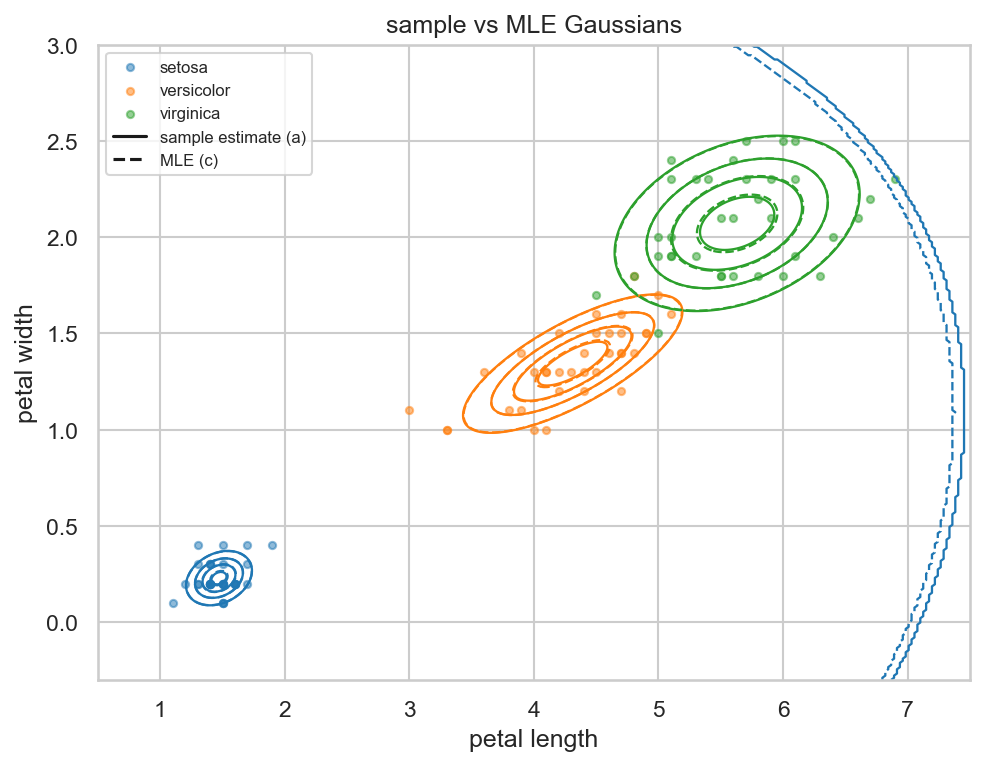
\includegraphics[width=0.55\linewidth]{figures/q2d_sample_vs_mle.png}
\caption{Sample-covariance Gaussians (solid) and MLE Gaussians (dashed). They almost coincide, the MLE ellipses being 1.4\% narrower ($\sqrt{0.971}$).}
\end{figure}

\textbf{e. Test performance.} The scratch MLE Bayes classifier gets a test error of \textbf{2.22\%} (one virginica predicted as
versicolor), the same as QDA in Q1, and it agrees with QDA on \textbf{100\%} of test predictions. This is expected, because both are
Gaussian class-conditional models with per-class covariances. The only difference is the $(n-1)/n$ factor, which scales every covariance by
nearly the same amount and so barely moves the boundaries.

\section*{Question 3 --- Naive Bayes for 20 Newsgroups}

11{,}269 training and 7{,}505 test documents, 20 classes, vocabulary of 61{,}188 words, given as \texttt{(docId, termId, count)} triples.
Everything is implemented with plain NumPy array operations (no ML library). Counts are accumulated directly from the
triples with \texttt{np.add.at}, so the dense $11\text{k}\times61\text{k}$ document--term matrix is never built.

\textbf{1. Training-set likelihood.} Multinomial Naive Bayes: $P(c)=N_c/N$, $P(w\mid c)=\text{count}(w,c)/\sum_{w'}\text{count}(w',c)$.
The training log-likelihood $\sum_d[\log P(c_d)+\sum_w n_{dw}\log P(w\mid c_d)]$ is \textbf{$-1.937\times10^{7}$}, i.e.\ $-7.01$ nats per word token.
It is finite because every word in a class-$c$ training document has, by construction, a non-zero count in class $c$.

\textbf{2. Laplace smoothing.} Without smoothing, 83.6\% of (class, word) pairs have zero count. On the test set, where 7{,}213 distinct
words never occurred in training at all, \textbf{92.7\% of documents get probability 0 under every class}, and accuracy collapses to 9.5\%
(no better than guessing). Laplace smoothing, $P(w\mid c) = (\text{count}(w,c)+1)/(\sum_{w'}\text{count}(w',c)+|V|)$, gives every word a
small non-zero probability in every class. As expected it lowers the training log-likelihood slightly (to $-2.021\times10^{7}$),
because some probability mass is moved to unseen words.

\textbf{3. \texttt{naiveBayesClassify}.} With $\alpha=1$ the test accuracy is \textbf{78.1\%}. A smaller smoothing constant works better:
accuracy peaks at \textbf{80.8\% for $\alpha=0.05$}. With a vocabulary of 61k words, $\alpha=1$ adds 61k pseudo-counts per class,
which is a large fraction of a class's real counts and flattens the distributions too much.

\begin{figure}[H]\centering
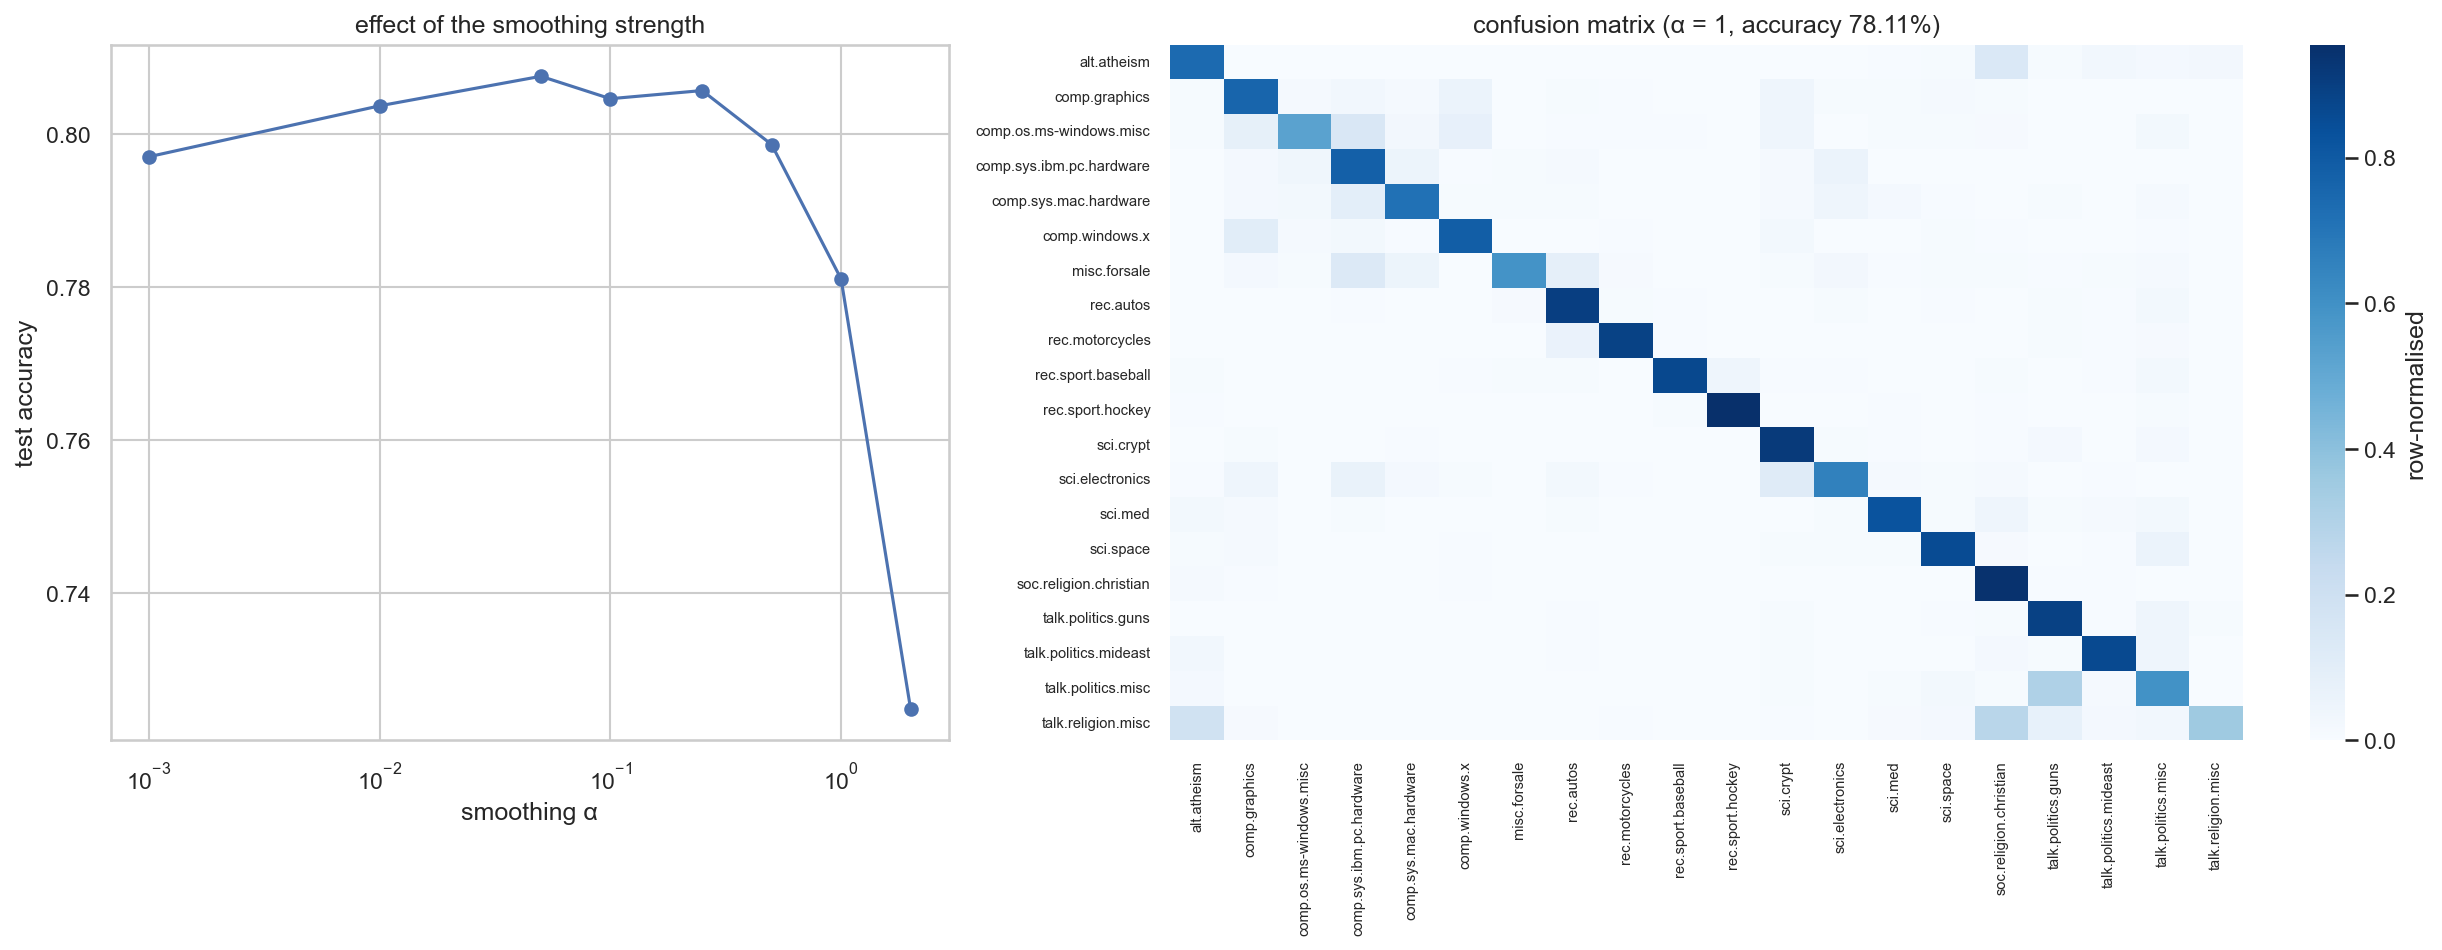
\includegraphics[width=\linewidth]{figures/q3_results.png}
\caption{Test accuracy vs.\ smoothing strength (left) and the row-normalised confusion matrix for $\alpha=1$ (right).}
\end{figure}

Per class, accuracy ranges from 95.5\% (rec.sport.hockey) and 94.7\% (soc.religion.christian), whose vocabularies are distinctive, down to
35.5\% (talk.religion.misc) and 52.9\% (comp.os.ms-windows.misc). The confusion matrix shows the errors stay inside related groups:
talk.religion.misc is absorbed by soc.religion.christian and alt.atheism, and the five \texttt{comp.*} hardware/OS groups confuse each other.
These groups share most of their vocabulary, so a bag-of-words model has little to separate them.

\end{document}
